\subsection{Dense Object Nets}
We implemented out training and benchmarking using ``PyTorch-Lightning''\cite{falcon2019pytorch} and ``PyTorch''\cite{paszke2019pytorch} libraries.
Futhermore, we employ
ADAM\cite{kingma2014adam} optimizer to optimize the model for 2500 epochs with learning rate of
$\alpha = 3 \times 10^{-4}, \beta_1 = 0.9 \text{ and } \beta_2 = 0.999$ with weight decay $\eta =10^{-4}$ to benchmark the DON with Pixelwise NT-Xent loss as in ~\cite{adrian2022efficient}
with a fixed batch size of 1 and 128 image-pair correspondences.
As per the benchmarking results in Table~\ref{table:don_training_results}, the robustness of the descriptor increases as the dimension of the descriptor gets longer.

\begin{table}[htb]
    \caption{Benchmark of DON framework for GPU consumption and AUC for $PCK@k,  \forall k \in [1, 100]$ metric.}
    \label{table:don_training_results}
    \centering
    \begin{tabular}{lllll}
        \toprule
        \multicolumn{5}{c}{DON benchmark}                                                                     \\
        \midrule
        Descriptor Size ($D$) & $3 $              & $8 $              & $4 $              & $32$              \\
        AUC for $PCK@k$       & $0.922 \pm 0.006$ & $0.933 \pm 0.011$ & $0.948 \pm 0.012$ & $0.953 \pm 0.008$ \\
        VRAM Usage (GB)       & $9.377 $          & $13.717 $         & $20.479 $         & $30.067$          \\
        \bottomrule
    \end{tabular}
\end{table}

The AUC for $PCK@k, \forall k \in [1, 100]$ is computed with 256 image-pair correspondences and
the mectric's mean and std. deviation is calculated from benchmarking 3 DON models trained for a single descriptor dimension.
We could not train the descriptor dimension of 64 and 128 due to the limited VRAM. Furthermore, to inspect the
results of trained DON, a interface is built using the PyGame library~\cite{pygame} to visualize the results of the trained DON.
The mouse pointer in image space is mapped to the pixel and the descriptor at that pixel is queried in an another image-descriptor space.
We further use the spatial probability of the descriptor to visualize the queried descriptor
in the image space using Equation~\ref{eqn:gaussian_kernel}
to identity if there are any multi-modal spatial activations in the descriptor spaces and there are none as shown in Figure~\ref{fig:check_don}.

\begin{figure}[htb]
    \centering
    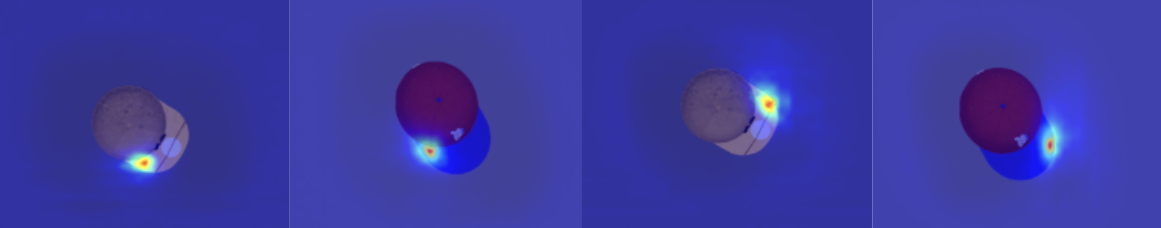
\includegraphics[scale=0.25]{images/test_don.png}
    \caption{Depiction of the spatial probability heatmaps of the descriptor in the image space. We set the temperature in the Equation~\ref{eqn:gaussian_kernel} to $1.1$
        and render the spatial probability heatmaps in the interface. The first and second image from the left and the right highlights the semantically equivalent descriptors in the image space.}
    \label{fig:check_don}
\end{figure}


\subsection{Our Framework}

To train our framework we employ ADAM optimizer to optimize the model for 2500 epochs with learning rate of
$\alpha = 1 \times 10^{-3}, \beta_1 = 0.9 \text{ and } \beta_2 = 0.999$ with no weight decay. We further use a fixed batch size of 1
and use StepLR scheduler with step size of 2500 and gamma of 0.9 to train the model. At first, we trained our model with 16 keypoints with
margin of 10 pixels as a hyperparameter for the separation loss and later we trained the models with 128 keypoints with margin of 2 pixels.


\begin{table}[htb]
    \caption{Benchmark of Our framework for GPU consumption and AUC for $PCK@k,  \forall k \in [1, 100]$ metric.}
    \label{table:framework_training_results}
    \centering
    \begin{tabular}{lllll}
        \toprule
        \multicolumn{5}{c}{Our framework with 16 keypoints}                                                   \\
        \midrule
        Descriptor Size ($D$) & $64 $             & $128 $            & $256 $            & $512$             \\
        AUC for $PCK@k$       & $0.922 \pm 0.006$ & $0.933 \pm 0.011$ & $0.948 \pm 0.012$ & $0.953 \pm 0.008$ \\
        VRAM Usage (GB)       & $9.377 $          & $13.717 $         & $20.479 $         & $30.067$          \\ \hline
        \multicolumn{5}{c}{Our framework with 128 keypoints}                                                  \\
        \midrule
        Descriptor Size ($D$) & $64 $             & $128 $            & $256 $            & $512$             \\
        AUC for $PCK@k$       & $0.922 \pm 0.006$ & $0.933 \pm 0.011$ & $0.948 \pm 0.012$ & $0.953 \pm 0.008$ \\
        VRAM Usage (GB)       & $9.377 $          & $13.717 $         & $20.479 $         & $30.067$          \\
        \bottomrule
    \end{tabular}
\end{table}